%卒論概要テンプレート ver. 4.0

\documentclass[uplatex,twocolumn,dvipdfmx]{jsarticle}
\usepackage[top=22mm,bottom=22mm,left=22mm,right=22mm]{geometry}
\setlength{\columnsep}{11mm}
\usepackage[T1]{fontenc}
\usepackage{txfonts}
\usepackage[expert,deluxe]{otf}
\usepackage[dvipdfmx,hiresbb]{graphicx}
\usepackage[dvipdfmx]{hyperref}
\usepackage{pxjahyper}
\usepackage{secdot}





%タイトルと学生番号,名前だけ編集すること
\title{\vspace{-5mm}\fontsize{14pt}{0pt}\selectfont Twitterのデマ拡散シュミレーション}
\author{\normalsize プロジェクトマネジメントコース 矢吹研究室 1442043 川崎貴雅}
\date{}
\pagestyle{empty}
\begin{document}
\fontsize{10.5pt}{\baselineskip}\selectfont
\maketitle



%以下が本文
\section{序論}\label{序論}

スマートフォンなどの普及と共にTwitterを始めとしたとしたマイクロブログが急激に普及している.Twitterはリアルタイムな情報を手軽に多くのユーザーへと伝播できるため社会に影響を与えている.例えば東日本大震災時のデマ情報が拡散された事や北朝鮮のミサイルを目撃したというデマが挙げられる.このようなツイートの拡散をシュミレーションで再現することを試みる.

本研究ではTwitterでのデマの拡散をシュミレーションで再現することができるかを調査したい.
実際にデマ拡散シュミレーションを行うために,人は1日にどのくらいツイートする数の確認とツイートが拡散する様子をシュミレートする手法の確立を行う.




\section{目的}

本研究ではシュミレーションを作成し,そのシュミレーションが現実のデマ拡散に近い状況を再現できるか調査することである.

\section{手法}

デマの拡散シュミレートするために以下の手順で行う.
\begin{enumerate}
\item TwitterAPIを用いて50万人のユーザーから1日のユーザー数にツイート数とフォロー数,フォロワー数の取得を行い,それをもとに1日の平均ツイート数を割り出す.
\item ツイートの拡散する様子をシュミレートする手法を確立するために,1から10までが0.2の確率でつながいってる図\ref{ランダムグラフ}のようなランダムグラフでのシュミレーションを試みる\cite{netto}.
\item 現実に近いシュミレーションにするために,上記2つを組み合わせたシュミレーションを行う.
\end{enumerate}
\begin{figure}[htb]
\centering
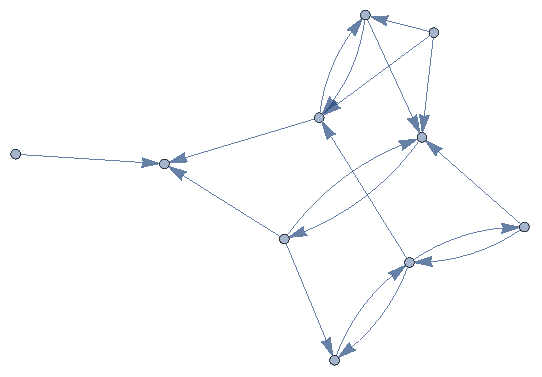
\includegraphics[width=44mm,clip]{graph.pdf}
\caption{使用したランダムグラフ}\label{ランダムグラフ}
\end{figure}
\section{結果}

50万人のデータから1日の平均ツイート数が1.37542回であることが分かった.またグループ構築にランダムグラフを使ったツイート拡散のシュミレート手法が確立できた.しかし平均ツイート数とツイート拡散のシュミレート手法を組み合わせた現実的なシュミレーションを行うことはできなかった.


\section{考察}

ランダムグラフを使ったシュミレーションは手法を確立させるにはよいが,現実的なシュミレーションを行うためには集めた50万人のデータをもとにシュミレーションを行うべきだと考えた.具体的にはフォロワー数の平均を割り出しシュミレーションへと反映させることで変わるのではないかと考えられる.

\section{結論}

本研究では,TwitterAPIで50万人のユーザーの1日のツイート平均数の算出とツイート拡散のシュミレートをする手法の確立を行った.その結果1日の平均ツイート数が1.37542回である事の確認,ツイートの拡散シュミレートの手法の確立が行えた.この結果を用いてシュミレーションを行うことでより現実的なシュミレーションを行えることが期待出来る.

\bibliographystyle{junsrt}
\bibliography{biblio}%「biblio.bib」というファイルが必要.

\end{document}
